\section{Results}
\label{sec:results}

\begin{table*}[t]
\centering
\small
\setlength{\tabcolsep}{4.2pt}
% generated by code/p9_table.py from the Phase 9 rows (contact cells marked \dagger: Phase 7d); do not edit by hand
\begin{tabular}{@{}lcccccccc@{}}
\toprule
 & \multicolumn{2}{c}{In distribution} & \multicolumn{2}{c}{Shift} & \multicolumn{2}{c}{Two-object contact} & \multicolumn{2}{c}{All three} \\
\cmidrule(lr){2-3}\cmidrule(lr){4-5}\cmidrule(lr){6-7}\cmidrule(l){8-9}
Pipeline & risk & cost & risk & cost & risk & cost & max gap & max cost \\
\midrule
\multicolumn{9}{@{}l}{\textit{Learned prior}} \\
PhysCtrl & \textcolor{gray}{0.130} & 0.05 & \textcolor{gray}{0.680} & 0.05 & \textcolor{gray}{0.693} & 0.10 & \textcolor{gray}{$+$0.722} & 0.10 \\
\multicolumn{9}{@{}l}{\textit{Fixed simulator setting}} \\
Coarse & \textcolor{gray}{0.040} & 0.13 & \textcolor{gray}{0.367} & 0.16 & \textcolor{gray}{0.318$^\dagger$} & 0.12$^\dagger$ & \textcolor{gray}{$+$0.367$^\dagger$} & 0.16$^\dagger$ \\
Tuned M1 & \textbf{0.015} & \textbf{0.13} & \textcolor{gray}{0.102} & 0.20 & \textbf{0.029} & \textbf{0.13} & \textcolor{gray}{$+$0.111} & 0.20 \\
Tuned M2 & 0.020 & 0.25 & \textcolor{gray}{0.102} & 0.29 & \textcolor{gray}{0.035} & 0.25 & \textcolor{gray}{$+$0.102} & 0.29 \\
Tuned M3 & 0.015 & 0.50 & \textcolor{gray}{0.155} & 0.51 & 0.000 & 0.50 & \textcolor{gray}{$+$0.155} & 0.51 \\
Reference (simulate all) & 0.000 & 1.00 & 0.000 & 1.00 & 0.000 & 1.00 & $+$0.000 & 1.00 \\
\multicolumn{9}{@{}l}{\textit{Gated}} \\
Seed-spread deferral & 0.000 & 1.11 & \textcolor{gray}{0.247} & 1.06 & \textcolor{gray}{0.086$^\dagger$} & 1.66$^\dagger$ & \textcolor{gray}{$+$0.247$^\dagger$} & 1.66$^\dagger$ \\
Momentum residual & 0.010 & 0.77 & 0.007 & 0.97 & \textcolor{gray}{0.290$^\dagger$} & 0.69$^\dagger$ & \textcolor{gray}{$+$0.290$^\dagger$} & 0.97$^\dagger$ \\
Certify or simulate & 0.015 & 0.54 & 0.003 & 0.87 & 0.000 & 1.18 & $+$0.015 & 1.18 \\
\midrule
\textbf{Ours} & 0.020 & 0.26 & \textbf{0.013} & \textbf{0.71} & 0.012 & 0.90 & \textbf{$+$0.025} & \textbf{0.90} \\
\bottomrule
\end{tabular}

\caption{\textbf{Every pipeline on the three test sets.}
Risk is the fraction of outputs with error above $\varepsilon = 0.10$; cost is compute per query relative to simulating it with the reference. Each object counts once.
Risks are against the reference at PhysCtrl's time step $\Delta t$, as pre-registered; \cref{tab:reference} repeats them against $\Delta t/2$ and $\Delta t/4$.
\emph{All three}: the largest gap to simulating every query, risk(pipeline) $-$ risk(reference at $\Delta t$), over the three sets and the three reference steps (defined after the Phase 10c verdict), and the largest cost.
Grey: risk above 0.03, or a gap above 0.03. Bold: the cheapest pipeline within 0.03 in each column.
M1--M3 are the reference solver at tuned cheaper settings. $^\dagger$: not run on this contact set; value from an earlier contact set (\cref{sec:res-contact}).}
\label{tab:main}
% src: results/p9_table (generated by code/p9_table.py from the Phase 9 rows; dagger cells from results/p7d_contact)
\end{table*}

\subsection{Main comparison}
\label{sec:res-main}
\Cref{tab:main} and \cref{fig:teaser}b compare all pipelines on the final test sets, each generated after the pipeline and its seven tests were fixed; all seven tests pass.
% src: Phase 9 (pre-registered Oct 19; verdicts results/p9_confirm, results/p9c_summary)

\paragraph{Ours tracks the simulator it replaces.}
Against the pre-registered reference, ours has risk 0.013 under shift at 0.71$\times$, saving 0.76\,s per query against certify-or-simulate (99\% CI [0.62, 0.91]) and 0.090 [0.055, 0.128] less risky than M1.
% src: Phase 9 C4, C5 (99% CIs, Bonferroni over five)
Re-scored against references at half and a quarter of the time step (\cref{sec:res-reference}), ours stays within 2.5 points of the risk of simulating every query on every set, the only pipeline below the simulator's cost to do so (\cref{tab:main}).
Each fixed setting is at least ten points riskier than the full simulator on some set: M1 and M3 under shift against every reference, coarse under shift, and M2 under shift against $\Delta t$; PhysCtrl fails everywhere outside its training regime.
The two other pipelines within the gap cost more than simulating on contact (certify-or-simulate 1.18$\times$) or are the simulator itself.
% src: Phase 10c (T3 for M1/M3, pre-registered; max gap, exploratory: results/p10c_explore)
The saving comes from the milder shifts: on the softer and stiffer families ours costs 0.50$\times$ and 0.24$\times$, while on 3$\times$ drag and drops almost every generation is rejected and ours costs as much as simulating (0.99$\times$, 1.10$\times$), as it should.
% src: Phase 9 per family (p9_confirm.assemble, Oct 20)

\paragraph{In distribution, safety has a price.}
Ours has risk 0.020 at 0.26$\times$ (99\% CI [0.21, 0.31]$\times$), 1.30\,s per query cheaper than certify-or-simulate ([1.03, 1.55]).
A tuned simulator is cheaper still (M1: 0.015 at 0.13$\times$), as we stated before the test; it stays safe only while the query resembles the data it was tuned on.
% src: Phase 9 C1-C3; pre-registration ("reported either way")

\subsection{The certificate}
\label{sec:res-cert}
On the final test sets the certificate accepted 1 of 272 bad generations under shift, 3 of 26 in distribution and 0 of 87 on contact; it is conservative, accepting 105 of 174 good generations in distribution and 1 of 45 on contact.
% src: results/p9_table (descriptive)
On the calibration objects the object-level guarantee held (false-accept rate 0.084, within the finite-sample bound of 0.11).
Under shift the window certificate let through 1.2\% of failures, whereas PhysCtrl's own uncertainty, the spread of eight samples, let through 35\% and accepted 99\% of the failed drops.
As a ranker of generation error (risk--coverage curves in the supplement) the window score has AUROC 0.977, against 0.886 for the momentum residual and 0.671 for seed spread, which is worse than random acceptance at low coverage; only a full coarse rollout ranks as well (0.973), at the cost of the rollout. The best of eight samples cannot fix shift: even the oracle choice is wrong for 68\% of shifted queries.
% src: Phase 4a extension (500 splits); 4m M1 (0.012; +0.341); 7a Q1, Q4 (development pool)

\subsection{Ablations}
\label{sec:res-ablation}
\begin{table}[t]
\centering
\footnotesize
\setlength{\tabcolsep}{3pt}
\begin{tabular}{@{}>{\raggedright\arraybackslash}p{3.55cm}>{\raggedright\arraybackslash}p{2.75cm}l@{}}
\toprule
Change & Effect & Source \\
\midrule
Restart the repair from generated positions, not the shadow's state & risk 0.017 $\to$ 0.070 & 4h vs.\ 4i \\
Restart at a shuffled chain point, not the first failure & error $+0.002$ [0.001, 0.003] & 4k \\
Uniform windows at matched budget & cost $+0.51$\,s (shift), $+1.24$\,s (in dist.); risk $-0.005$ & 4m \\
Three windows instead of one (single objects) & AUROC 0.958 vs.\ 0.955 at 3$\times$ the probe cost & E2$^*$ \\
One window instead of three (contact) & risk 0.012 $\to$ 0.095 & 4o$^\circ$ \\
Switch timed by the generation, not the shadow & risk 0.012 $\to$ 0.025 & Ph.~9 \\
Restart at the first failing window, not the shadow-timed switch & same risk; error 0.015 $\to$ 0.029, cost 0.90 $\to$ 0.67 & Ph.~9 \\
Windows placed at the predicted contact & captures less error than uniform & 4l \\
Reference-setting suffix instead of the medium one & cost 25--55\% higher at similar risk & 8a$^*$ \\
Repair with the generator (5 variants) & error at most 1\% lower & 4b--4g \\
\bottomrule
\end{tabular}
\caption{\textbf{What each component buys.} Each row changes one component, in the pre-registered phase named in the last column (test sets differ between rows). $^*$exploratory, development data; $^\circ$code check on seen scenes before the final test.}
\label{tab:ablation}
% src: PLAN.md phases as listed; Phase 9 rows from results/p9c_summary
\end{table}
\Cref{tab:ablation} isolates the components.
The shadow's full state is what makes repair work: a restart from generated positions loses the stress state and the drift, and fails.
On contact, the shadow-timed switch halves the error of the plain chain repair and is safer than a switch timed by the generation, whose contact is itself wrong; the plain chain repair is cheaper at the same risk, so the switch buys accuracy rather than a lower risk.
A single window suffices for one object but misses ignored collisions, which is why contact scenes keep three.

\subsection{Two-object contact}
\label{sec:res-contact}
PhysCtrl generates each object as if it were alone, and 69\% of composed contact scenes are wrong.
Ours has risk 0.012 against 0.000 for certify-or-simulate and saves 1.31\,s per scene ([1.03, 1.60]), at 0.90$\times$ the cost of simulation; on an earlier set of fresh scenes the switch was confirmed in the same way.
% src: Phase 9 CC1-CC3; Phase 4o
The cheap shortcuts fail on contact: coarse simulation has risk 0.318, because the coarse grid cannot resolve the gap between the objects, and the momentum-residual gate 0.290, because a collision between two objects leaves the total momentum unchanged, as we predicted before the data.
% src: Phase 7d (on the 4o scenes)
Tuned simulators are cheaper on contact (M3 0.000 at 0.50$\times$; M1 0.029 at 0.13$\times$, 4 bad scenes of 132), but under shift both are about ten points riskier than the full simulator against every reference step.
% src: Phase 10c T3 (M1 +0.09 to +0.12, M3 +0.11 to +0.14)

\subsection{Is the reference converged?}
\label{sec:res-reference}
As in PhysCtrl's own evaluation, ground truth is the MPM simulator that produced its training data, so we test that reference.
Before the object reaches the floor, the drop ground truth falls as $\tfrac12 g t^2$ predicts (centre of mass within $1.2{\times}10^{-4}$ over 78 queries).
% src: Phase 10a R3 (amended contact layer: two grid cells)
Halving the time step, however, moves the reference by a 95th-percentile distance of 0.026 in distribution, 0.044 on contact and 0.009 for stiffer materials, but by 0.20, 0.12 and 0.43 for softer materials, drops and stronger pushes; a quarter step moves it further.
For 21\%, 7\% and 18\% of the queries in those three families the reference itself moves by more than our error bound, so the reference is not converged at our scale there, and risk comparisons on them inherit this uncertainty.
% src: results/p10a_convergence (job 96); R1 fails except for the stiffer family; R2 fails

\begin{table*}[t]
\centering
\small
\setlength{\tabcolsep}{4.2pt}
% generated by code/p10c_table.py from results/p10c_summary and results/p10c_explore; do not edit by hand
\begin{tabular}{@{}lcccccccccc@{}}
\toprule
 & \multicolumn{3}{c}{In distribution} & \multicolumn{4}{c}{Shift} & \multicolumn{3}{c}{Two-object contact} \\
\cmidrule(lr){2-4}\cmidrule(lr){5-8}\cmidrule(l){9-11}
Reference step & $\Delta t$ & $\Delta t/2$ & $\Delta t/4$ & $\Delta t$ & $\Delta t/2$ & $\Delta t/4$ & robust & $\Delta t$ & $\Delta t/2$ & $\Delta t/4$ \\
\midrule
PhysCtrl & 0.130 & 0.110 & 0.100 & 0.680 & 0.665 & 0.650 & 0.647 & 0.693 & 0.722 & 0.737 \\
Tuned M1 & 0.015 & 0.025 & 0.025 & 0.102 & 0.224 & 0.329 & 0.102 & 0.029 & 0.029 & 0.082 \\
Tuned M2 & 0.020 & 0.020 & 0.015 & 0.102 & 0.099 & 0.226 & 0.048 & 0.035 & 0.023 & 0.041 \\
Tuned M3 & 0.015 & 0.030 & 0.030 & 0.155 & 0.232 & 0.324 & 0.157 & 0.000 & 0.019 & 0.130 \\
Reference at $\Delta t$ & 0.000 & 0.005 & 0.020 & 0.000 & 0.113 & 0.226 & 0.000 & 0.000 & 0.000 & 0.037 \\
Certify or simulate & 0.015 & 0.020 & 0.030 & 0.003 & 0.116 & 0.226 & 0.000 & 0.000 & 0.000 & 0.037 \\
\midrule
\textbf{Ours} & 0.020 & 0.025 & 0.030 & 0.013 & 0.108 & 0.216 & 0.005 & 0.012 & 0.012 & 0.062 \\
\bottomrule
\end{tabular}

\caption{\textbf{Every pipeline re-scored against the reference at three time steps} (Phase 9 test sets; risk = fraction with error above 0.10, each object counted once).
$\Delta t$ is PhysCtrl's step, against which \cref{tab:main} is scored; $\Delta t/4$ was pre-registered as the primary reference for this table.
\emph{Robust}: wrong against all three references (defined after the verdict).
--: not run on this set.}
\label{tab:reference}
% src: results/p10c_summary (pre-registered, job 101), results/p10c_explore (robust; exploratory)
\end{table*}

We therefore re-scored every pipeline exactly against the reference at $\Delta t/2$ and $\Delta t/4$ (\cref{tab:reference}; pre-registered).
PhysCtrl is riskier than ours in every set against every reference (98.3\% CIs; under shift 0.650 vs.\ 0.216 against $\Delta t/4$).
Absolute risk, however, depends on the reference: under shift, simulating every query at $\Delta t$ is itself wrong for 11\% and 23\% of queries against the finer references, as is ours (11\%, 22\%), so the pre-registered bound of 0.03 holds against $\Delta t$ only; on contact against $\Delta t/4$, ours has 0.062 and simulating every query 0.037.
Relative to simulating every query, ours stays within $+$0.025 everywhere, and 0.5\% of its shifted outputs are wrong against all three references, against 10\%, 4.8\% and 16\% for M1--M3 (exploratory).
M1 and M3 are riskier than ours under shift against every reference; M2 is not (against $\Delta t/4$ its risk equals the full simulator's), so it is as safe as ours under shift within the reference's uncertainty, at 0.29$\times$ instead of 0.71$\times$, though without a per-query signal.
% src: results/p10c_summary (T1 PASS, T2 FAIL, T3 M1/M3 PASS, M2 FAIL); results/p10c_explore

\subsection{PhysCtrl's own metrics}
\label{sec:res-physctrl}
\begin{table}[t]
\centering
\footnotesize
\setlength{\tabcolsep}{3.5pt}
\resizebox{\linewidth}{!}{%
\begin{tabular}{@{}lccccc@{}}
\toprule
 & vIoU $\uparrow$ & CD $\downarrow$ & MSE $\downarrow$ & risk & cost \\
\midrule
PhysCtrl, reported~\cite{wang2025physctrl} & 77.59\% & 0.0028 & 0.0015 & -- & -- \\
PhysCtrl, our run & 77.57\% & 0.0028 & 0.0015 & 0.220 & 0.05 \\
Certify or simulate & 92.20\% & 0.0006 & 0.0003 & 0.030 & 0.57 \\
\textbf{Ours} & 86.81\% & 0.0008 & 0.0004 & 0.030 & 0.24 \\
\bottomrule
\end{tabular}}
\caption{\textbf{PhysCtrl's 100-object test set and metrics}, computed with PhysCtrl's own evaluation code; PhysCtrl reports 25 sampling steps, we sample with 4. Development data (descriptive).}
\label{tab:physctrl}
% src: Phase 10b (job 97) + PhysCtrl's volume_iou.py; reported row from PhysCtrl Table 2
\end{table}
Run through PhysCtrl's own evaluation code, our generations reproduce its reported numbers (vIoU 77.57\% vs.\ 77.59\%, Chamfer 0.0028, MSE 0.0015), so our setup matches its protocol; yet 22\% of these in-distribution trajectories exceed our error bound.
% src: results/p7b_testset_volume (PhysCtrl's volume_iou.py on the 7b outputs); results/p7b_testset (risk 0.220)
With our certificate and repair, vIoU rises to 86.81\% and the Chamfer distance falls 3.5$\times$, at a quarter of the cost of simulating; certifying and simulating rejected queries in full is closer still (92.20\%) at 0.57$\times$.
% src: results/p10b_testset (job 97, final pipeline)

\subsection{What did not work}
\label{sec:res-negative}
Optimising the generation against the window defect lowered the defect while nearly doubling the true error (0.267 to 0.511): the defect is a certificate, not an objective. Other negative results (cheap-simulator certification, stiff materials, amortisation) are in the supplement.
% src: Phase 4c; pilots 8d, E1/E1b; 5a

\subsection{Qualitative results}
\label{sec:res-qual}
\begin{figure}[t]
\centering
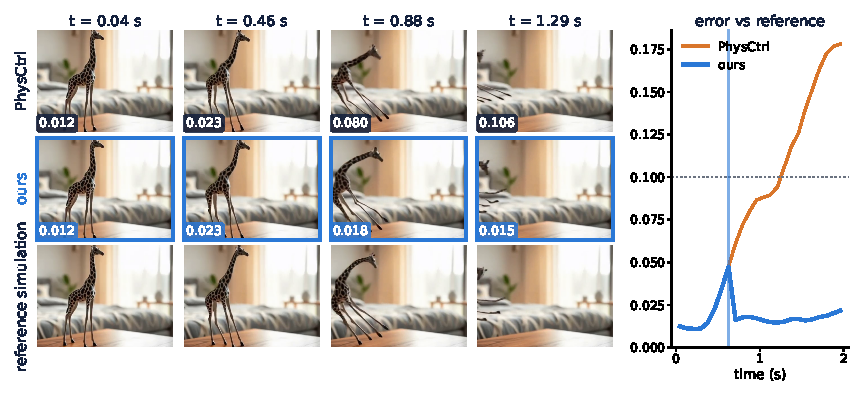
\includegraphics[width=\linewidth]{fig/qual_video.pdf}
\caption{\textbf{Rendered video} of PhysCtrl's giraffe example with 3$\times$ its drag force, chosen by the rule fixed before rendering (median PhysCtrl error among rejected cases). Labels: per-frame error. Our check fails at frame 7 and the rest is re-simulated.}
\label{fig:qual-video}
% src: job 95 (Phase 9 pipeline); results/fig_qualitative/paper_video_selection.json
\end{figure}
PhysCtrl fails on contact because it ignores the collision: on the two rule-selected contact scenes its composed output nearly coincides with the two objects simulated apart (error 0.136 vs.\ 0.119, and 0.125 vs.\ 0.112), while ours follows the reference to 0.028 and 0.025 (\cref{fig:teaser}a; both scenes in the supplement).
% src: job 94 (paper_contact_*.npz)
On PhysCtrl's five image examples with 3$\times$ their drag force, our check rejected all five and the repair lowered the error 1.8--18$\times$ (from 0.061--0.222 to 0.013--0.034); with the forces as given, all five were accepted (\cref{fig:qual-video}).
% src: job 95, case_v2.json (blanket 0.089->0.031, chair 0.061->0.034, earphone 0.222->0.013, giraffe 0.086->0.018, penguin 0.073->0.030)
Shifted queries, both contact scenes and all ten videos are in the supplement.
